\documentclass{standalone}
\usepackage{calc}
\usepackage{tikz}

\begin{document}
	\begin{tikzpicture}[scale = 0.25, very thin]
	
		% Tiles
%		\foreach \x in {0,...,2} {
%			\foreach \y in {0,...,2}{
%				\fill[gray, opacity = 0.5] (\x * 5, -\y * 5) rectangle ++(7, -7);
%			}
%		}

		% Summed up masks
		\node<1>[anchor = north west, inner sep = 0] at (0, 0) {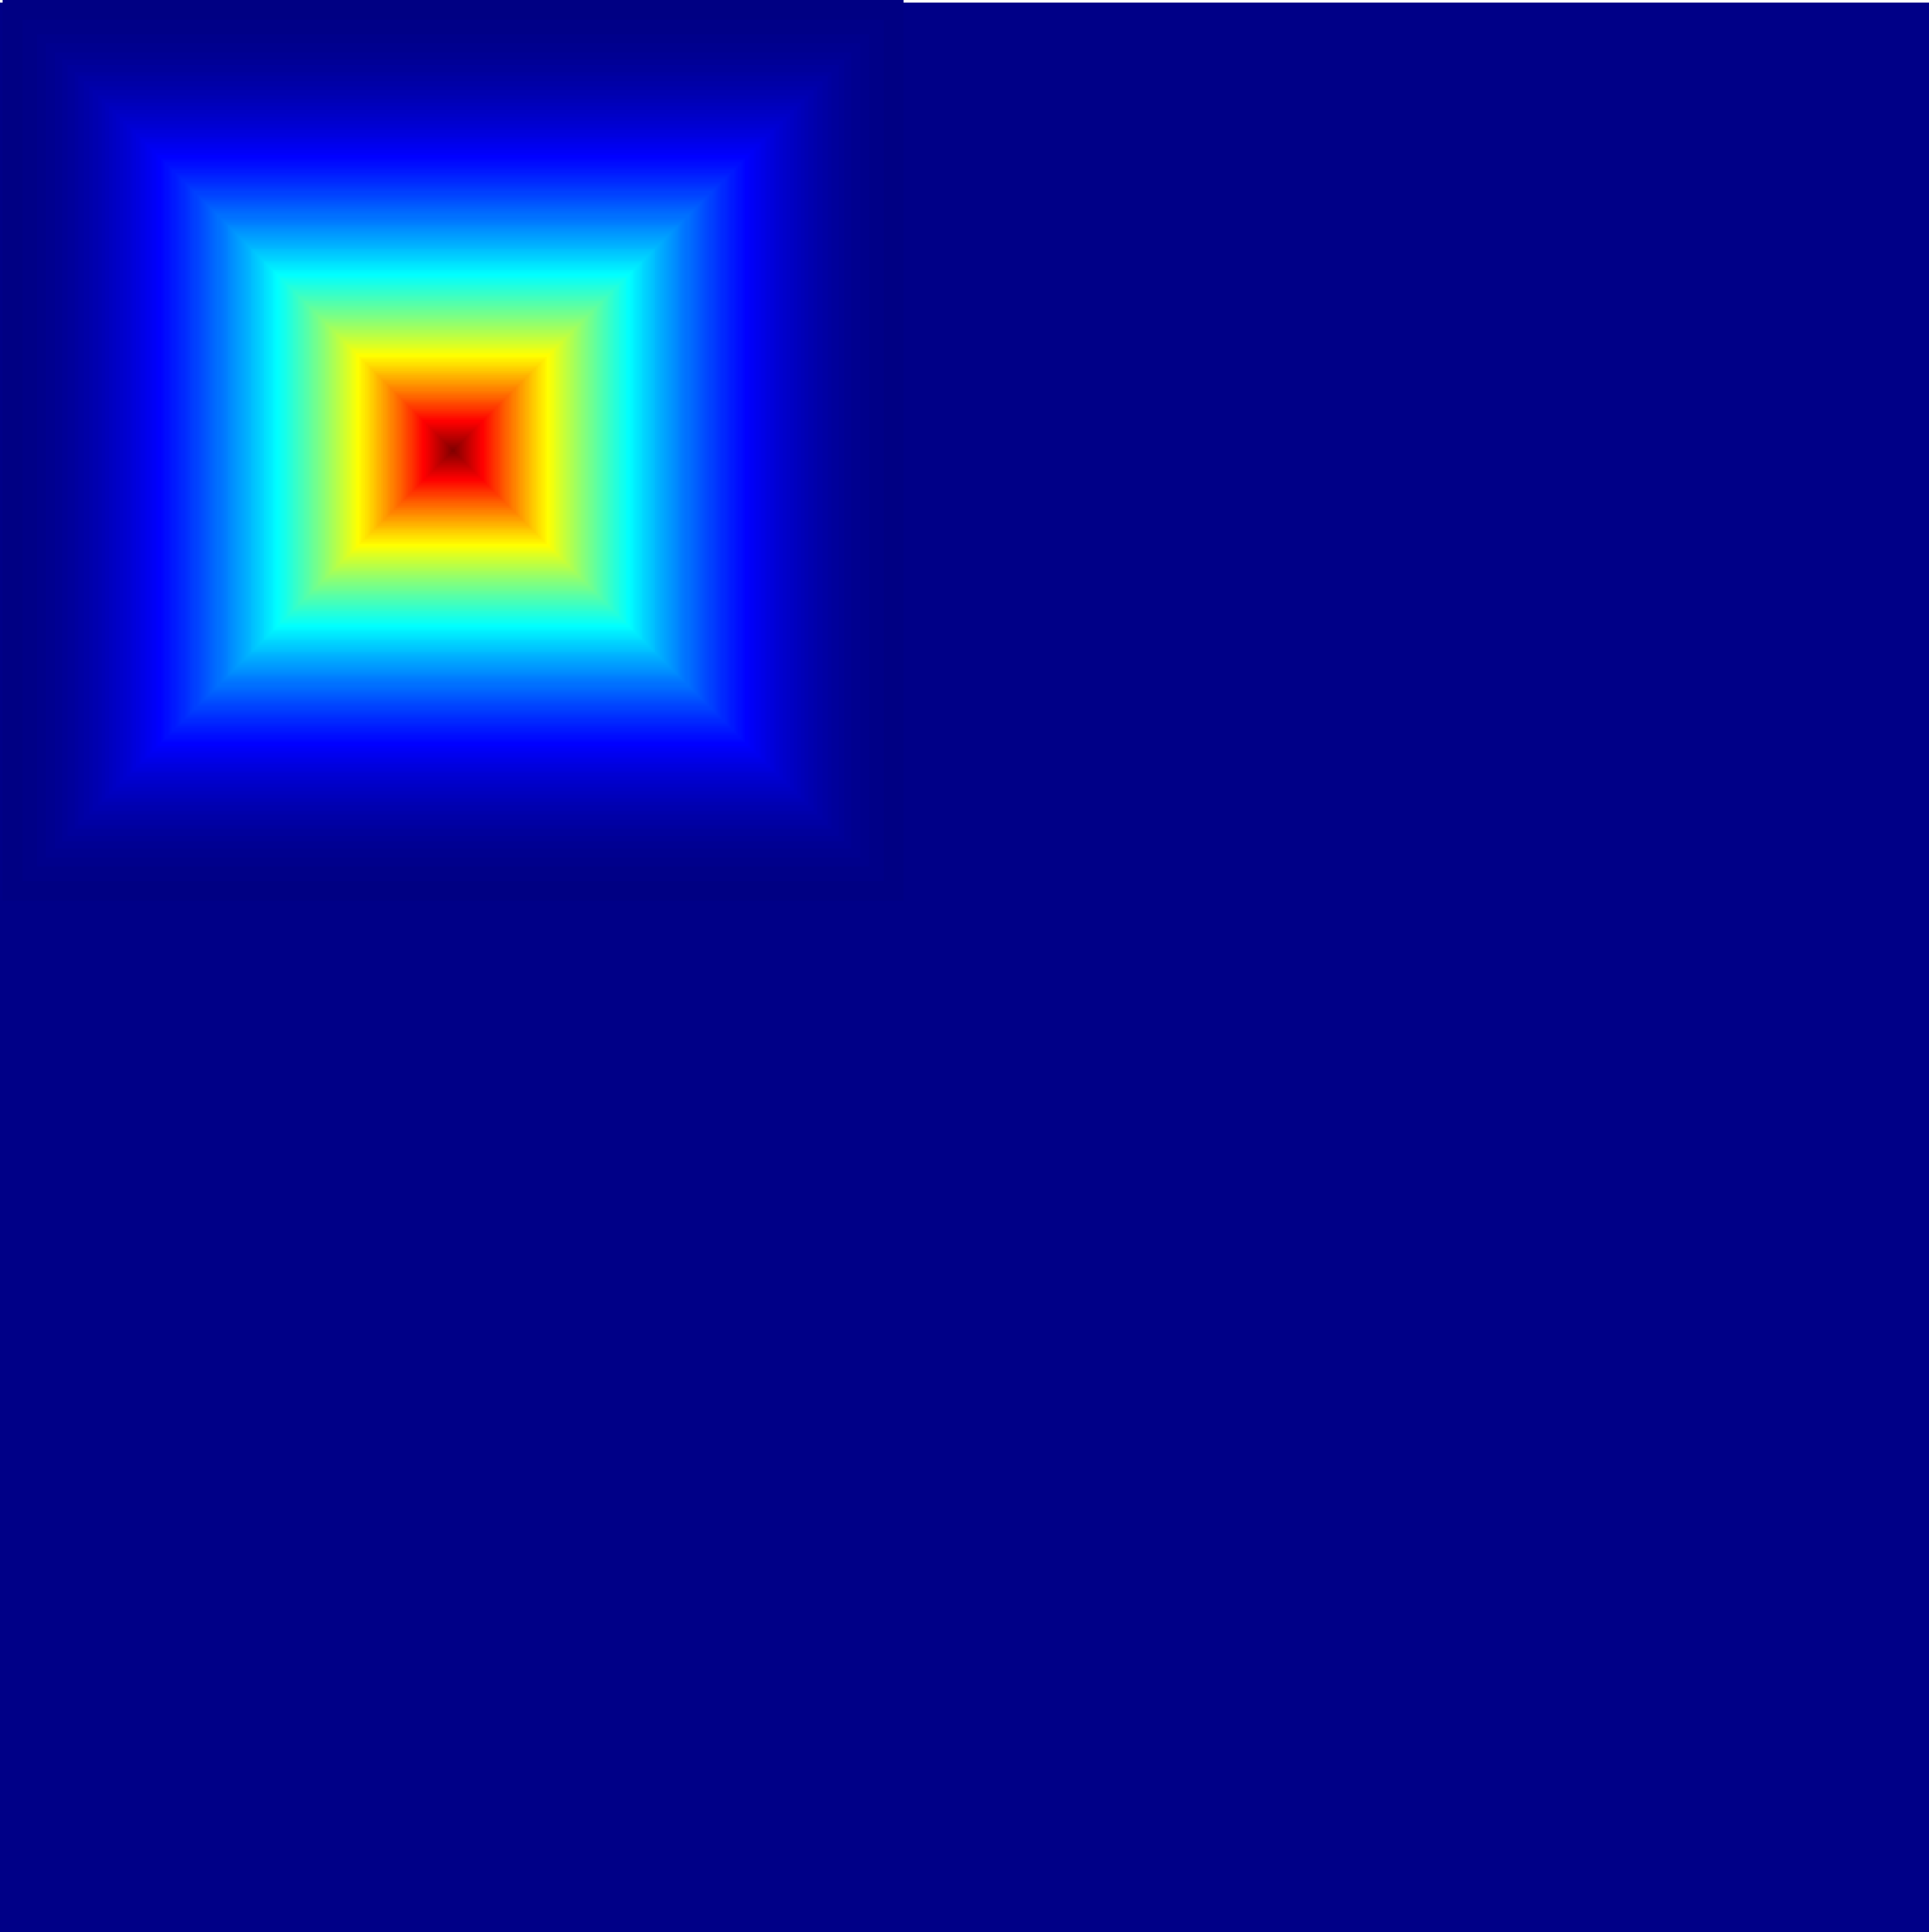
\includegraphics[width = 3.75cm]{./figures/tiling/mask1}};
		\node<2>[anchor = north west, inner sep = 0] at (0, 0) {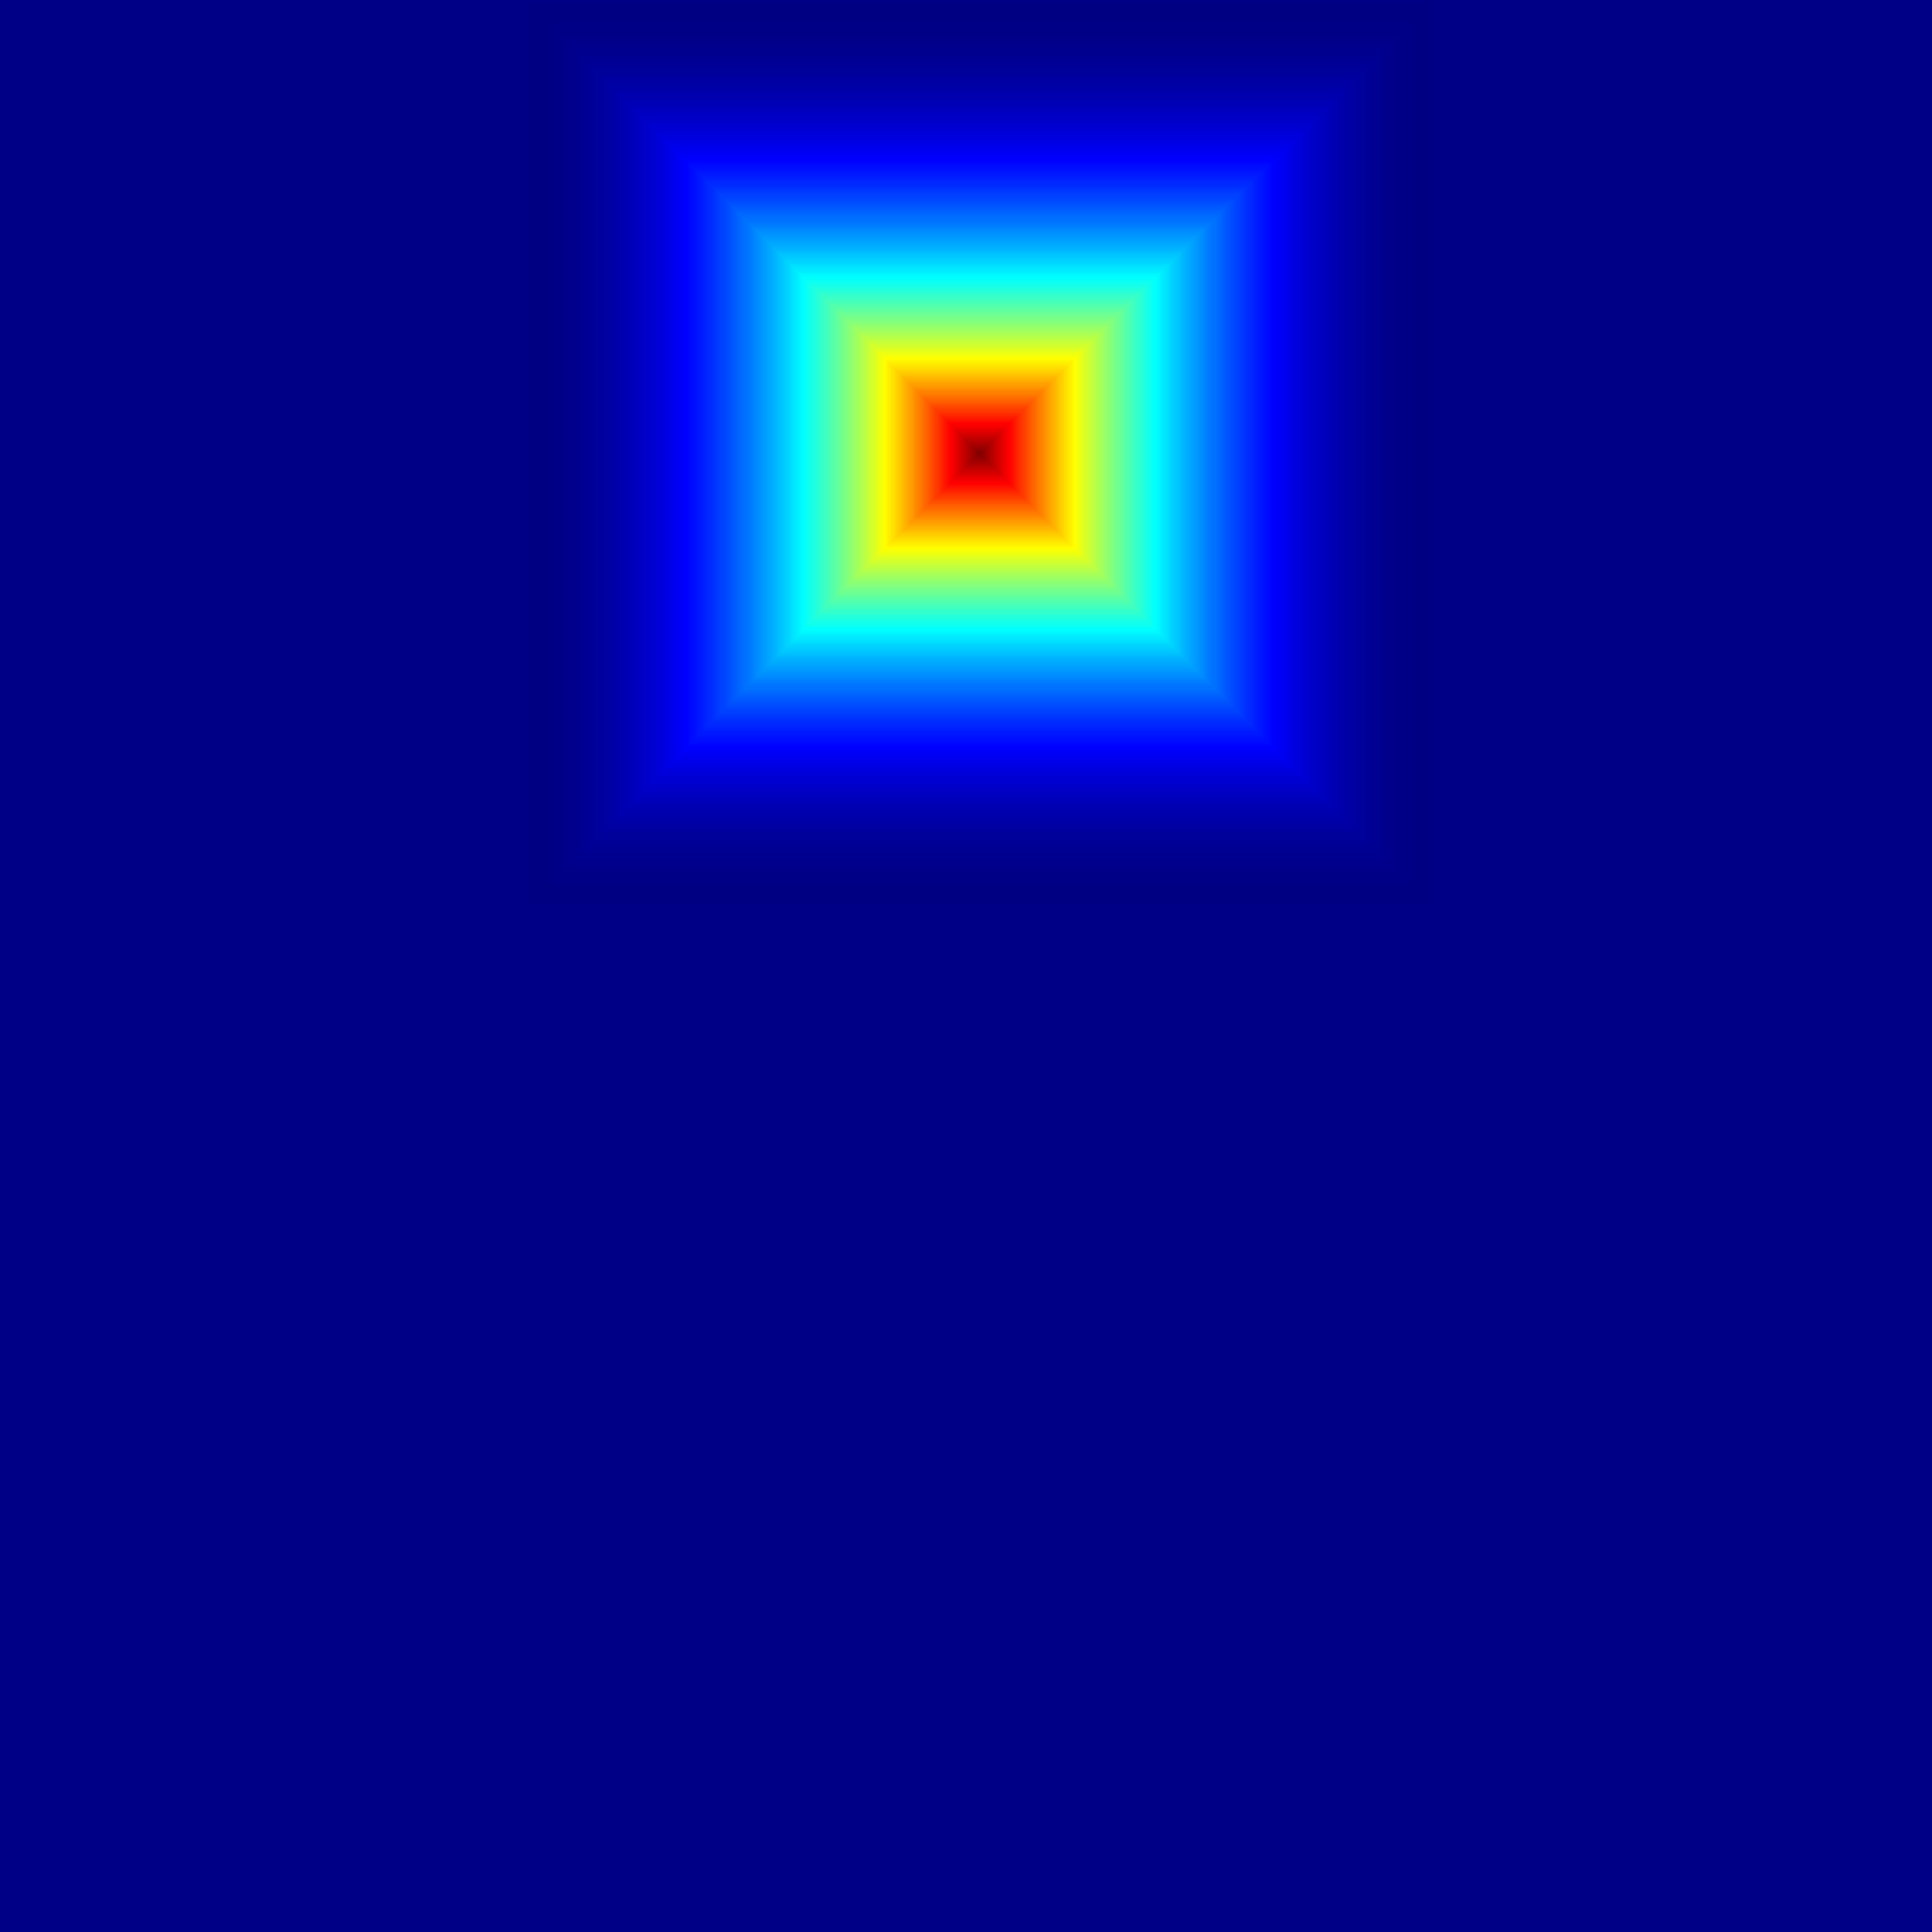
\includegraphics[width = 3.75cm]{./figures/tiling/mask2}};
		\node<3>[anchor = north west, inner sep = 0] at (0, 0) {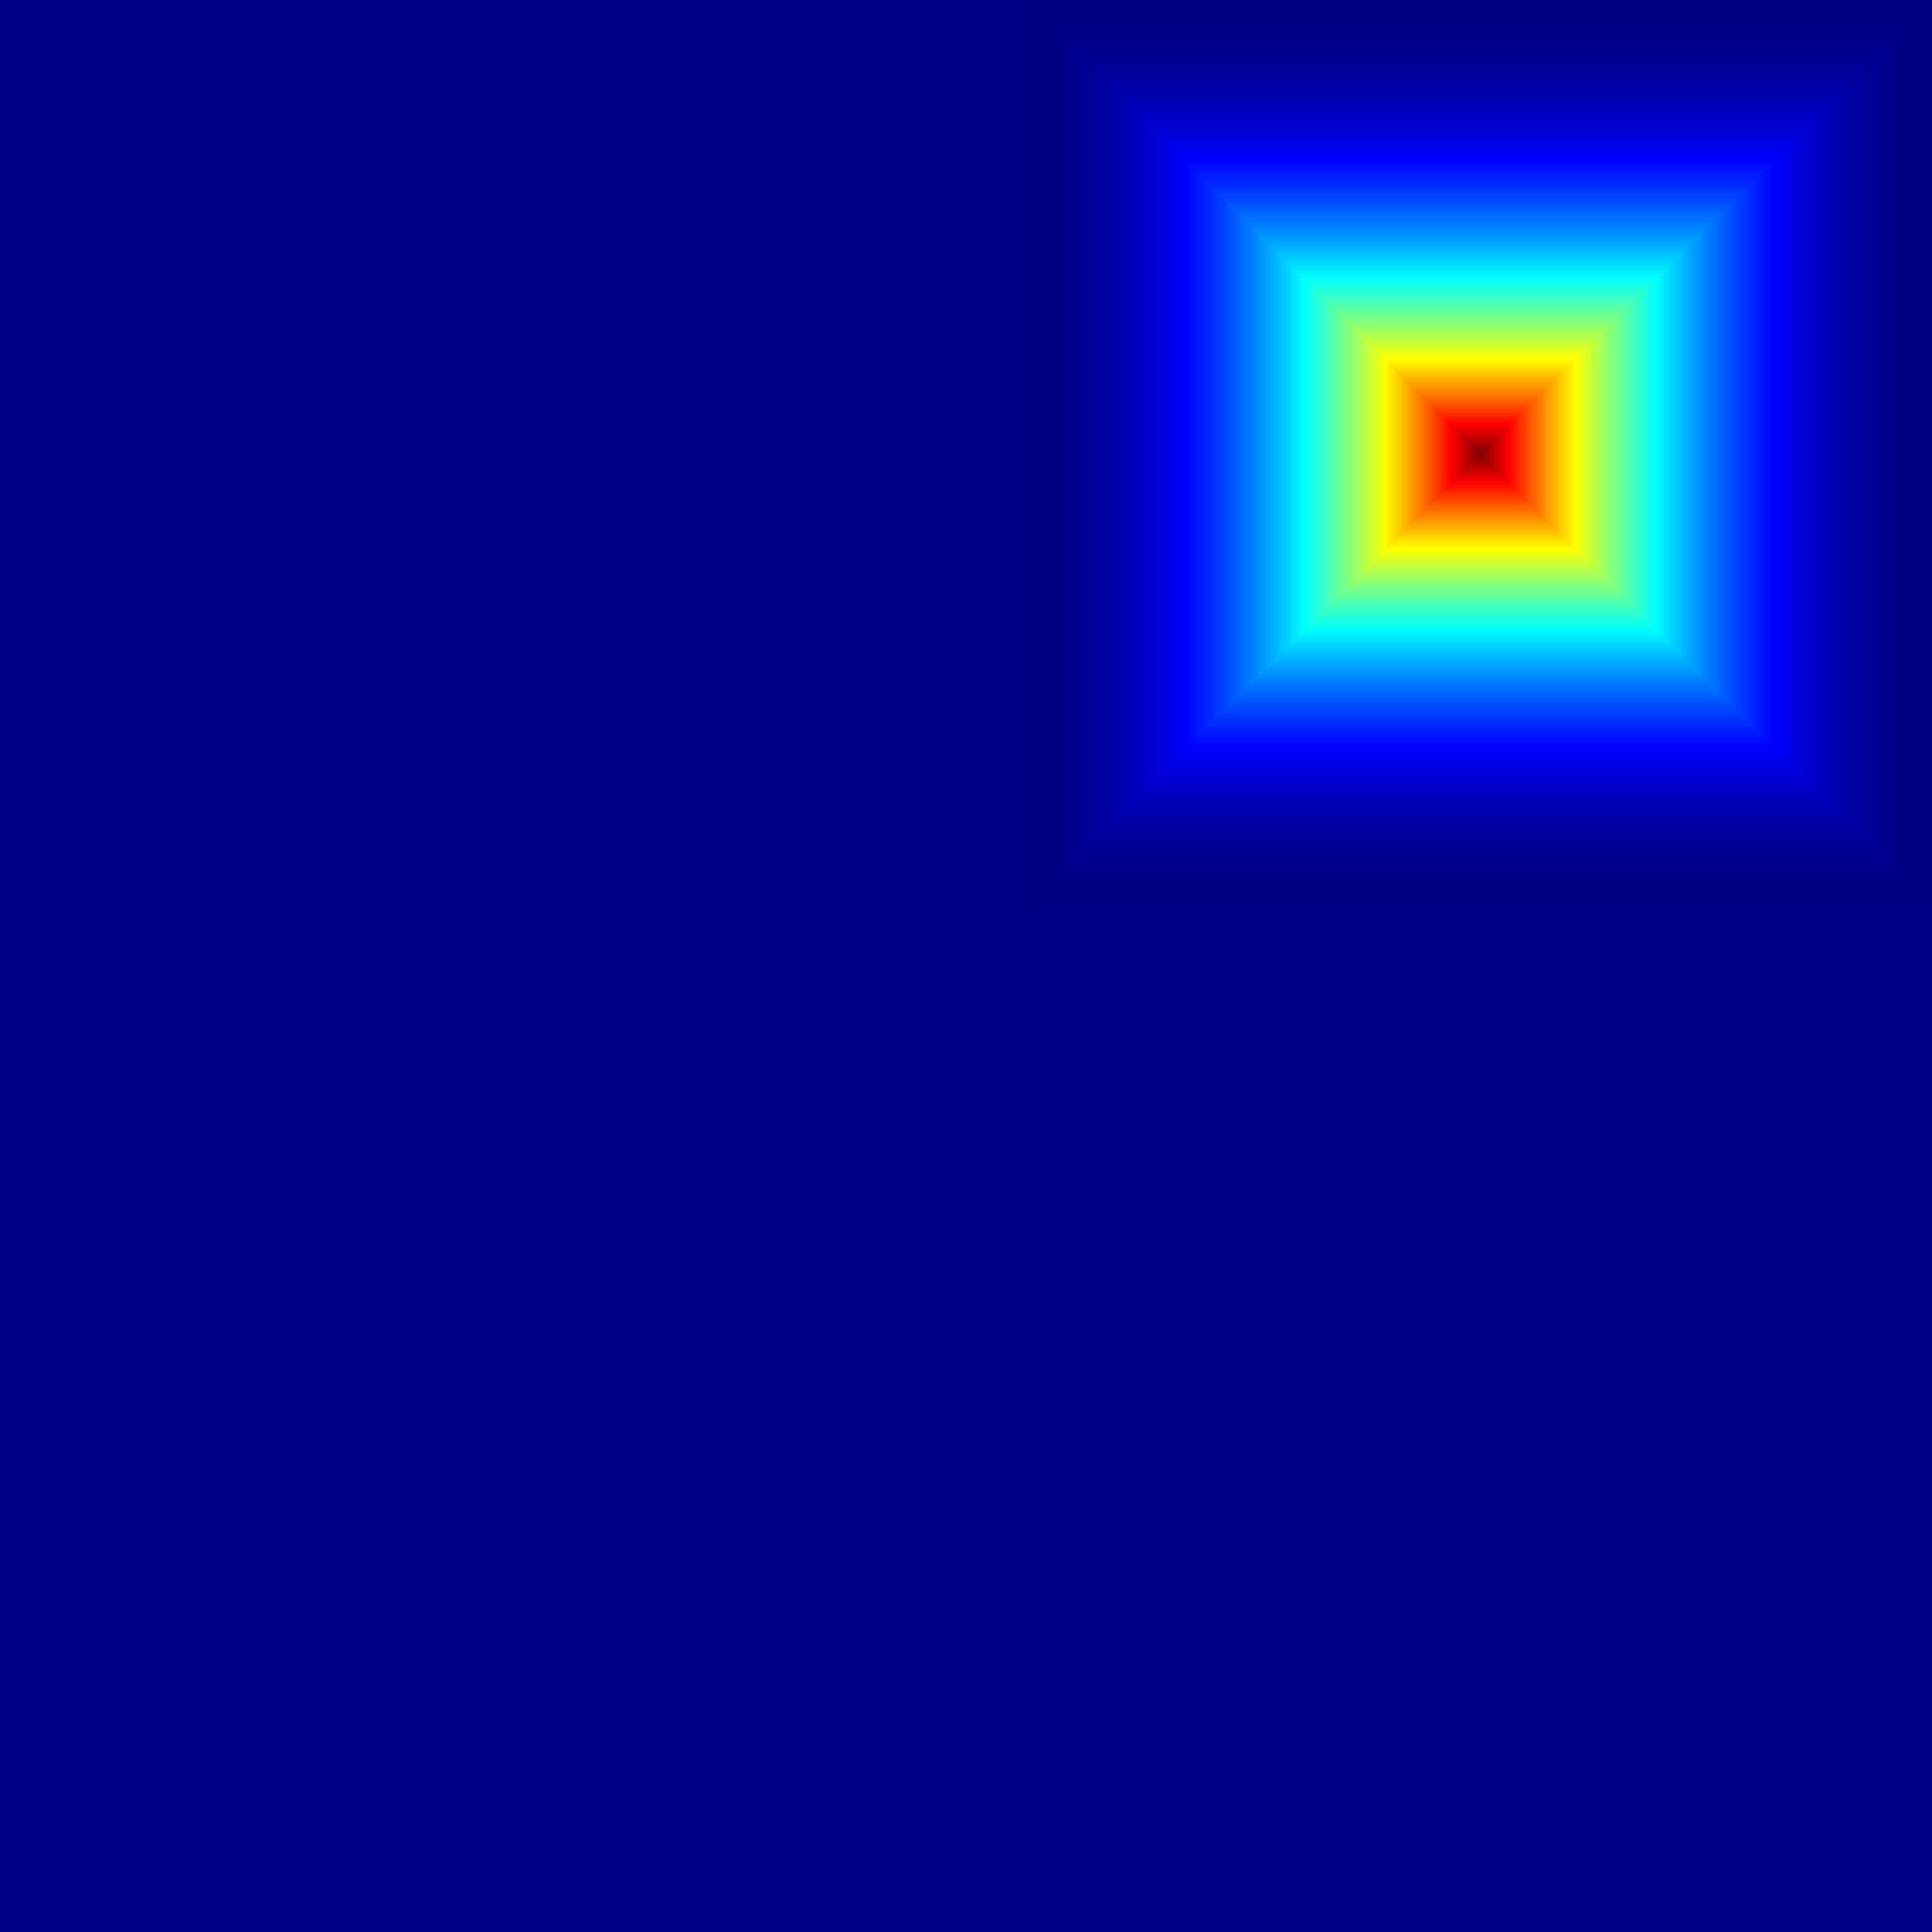
\includegraphics[width = 3.75cm]{./figures/tiling/mask3}};
		\node [anchor = east, scale=2] at (-0.5, -7.5) {$\ast$};
		% Grid
%		\draw[step = 1 cm, cap = round] (0, 0) grid (15, -15);
		
		% Invisible markers for accurate placement in figure 
		\begin{scope}[opacity = 0]
			\draw[|-|] (0, -18) -- node[below]	{$R_x$} ++(15, 0);
%			\draw[|-|] (18, 0) -- node[right]	{$R_y$} ++(0, -15);
			\draw[|-|] (0, 1) 	-- node[above]	{$r_x$} ++(7, 0);
%			\draw[|-|] (-1, 0) 	-- node[left]	{$r_y$} ++(0, -7);
			\draw[|-|] (10, 1) 	-- node[above]	{$o_x$} ++(2, 0);
%			\draw[|-|] (-1, -10) -- node[left]	{$o_y$} ++(0, -2);
		\end{scope}
		
	\end{tikzpicture}
\end{document}